\hypertarget{mrisystemphantom.jl-digital-twin-library}{%
\chapter{MRISystemPhantom.jl --- Digital Twin
Library}\label{ch:mri-system-phantom}}

%%%%%%%%%%%%%%%%%%%%%%%%%%%%%%%%%%%%%%%
% IMPORTANT
\begin{spacing}{1} %THESE FOUR
\minitoc % LINES MUST APPEAR IN
\end{spacing} % EVERY
\thesisspacing % CHAPTER
% COPY THEM IN ANY NEW CHAPTER
%%%%%%%%%%%%%%%%%%%%%%%%%%%%%%%%%%%%%%%

\hypertarget{the-physical-phantom}{%
\section{The physical phantom}\label{the-physical-phantom}}

The QalibreMD NIST/ISMRM
\href{https://qmri.com/product/premium-system-phantom/}{System Standard
Model 130} (manufactured by \href{https://qmri.com}{Caliber MRI},
formerly QalibreMD) is a hardware phantom designed to mimic the geometry
of a human head and to provide a wide, calibrated range of quantitative
MRI tissue parameters (T1, T2, and proton density). It is the standard
reference device for quantitative MRI system validation in clinical and
research settings, and its design is described in the \emph{QalibreMD
System Standard Model 130 User Manual}
(\href{https://github.com/ArthurAllilaire/RLxMRI/blob/main/QalibreMD_NIST_ISMRM_System_Standard_Model_130_T1_T2_PD_User_Manual.pdf}{available
here}).

The phantom consists of a spherical water-filled housing (100 mm
internal radius) containing four internal structures at fixed axial
positions:

\begin{longtable}[]{@{}lll@{}}
\toprule
\begin{minipage}[b]{0.26\columnwidth}\raggedright
Plate\strut
\end{minipage} & \begin{minipage}[b]{0.29\columnwidth}\raggedright
z (mm)\strut
\end{minipage} & \begin{minipage}[b]{0.37\columnwidth}\raggedright
Contents\strut
\end{minipage}\tabularnewline
\midrule
\endhead
\begin{minipage}[t]{0.26\columnwidth}\raggedright
T1 array\strut
\end{minipage} & \begin{minipage}[t]{0.29\columnwidth}\raggedright
+56.5\strut
\end{minipage} & \begin{minipage}[t]{0.37\columnwidth}\raggedright
14 NiCl\(_2\) spheres (15 mm radius), T1 range \textasciitilde24 ms -- 1.9 s
at 3 T\strut
\end{minipage}\tabularnewline
\begin{minipage}[t]{0.26\columnwidth}\raggedright
T2 array\strut
\end{minipage} & \begin{minipage}[t]{0.29\columnwidth}\raggedright
+16.5\strut
\end{minipage} & \begin{minipage}[t]{0.37\columnwidth}\raggedright
14 MnCl\(_2\) spheres (15 mm radius), T2 range \textasciitilde87 ms -- 2.8 s
at 3 T\strut
\end{minipage}\tabularnewline
\begin{minipage}[t]{0.26\columnwidth}\raggedright
PD array\strut
\end{minipage} & \begin{minipage}[t]{0.29\columnwidth}\raggedright
-23.5\strut
\end{minipage} & \begin{minipage}[t]{0.37\columnwidth}\raggedright
14 spheres of varying proton density (15 mm radius)\strut
\end{minipage}\tabularnewline
\begin{minipage}[t]{0.26\columnwidth}\raggedright
Fiducial grid\strut
\end{minipage} & \begin{minipage}[t]{0.29\columnwidth}\raggedright
distributed\strut
\end{minipage} & \begin{minipage}[t]{0.37\columnwidth}\raggedright
57 small spheres (5 mm radius) on a 40 mm cubic lattice\strut
\end{minipage}\tabularnewline
\bottomrule
\end{longtable}

Each contrast plate arranges its 14 spheres in two concentric rings: 10
on an outer ring of radius 65 mm and 4 on an inner ring of radius 28 mm.
This geometry matches the phantom manual photographs but has not been
verified against the physical device. The current digital twin models
the contrast arrays and fiducial grid, but not the resolution insets or
the two slice-profile wedges.

\begin{figure}
\centering
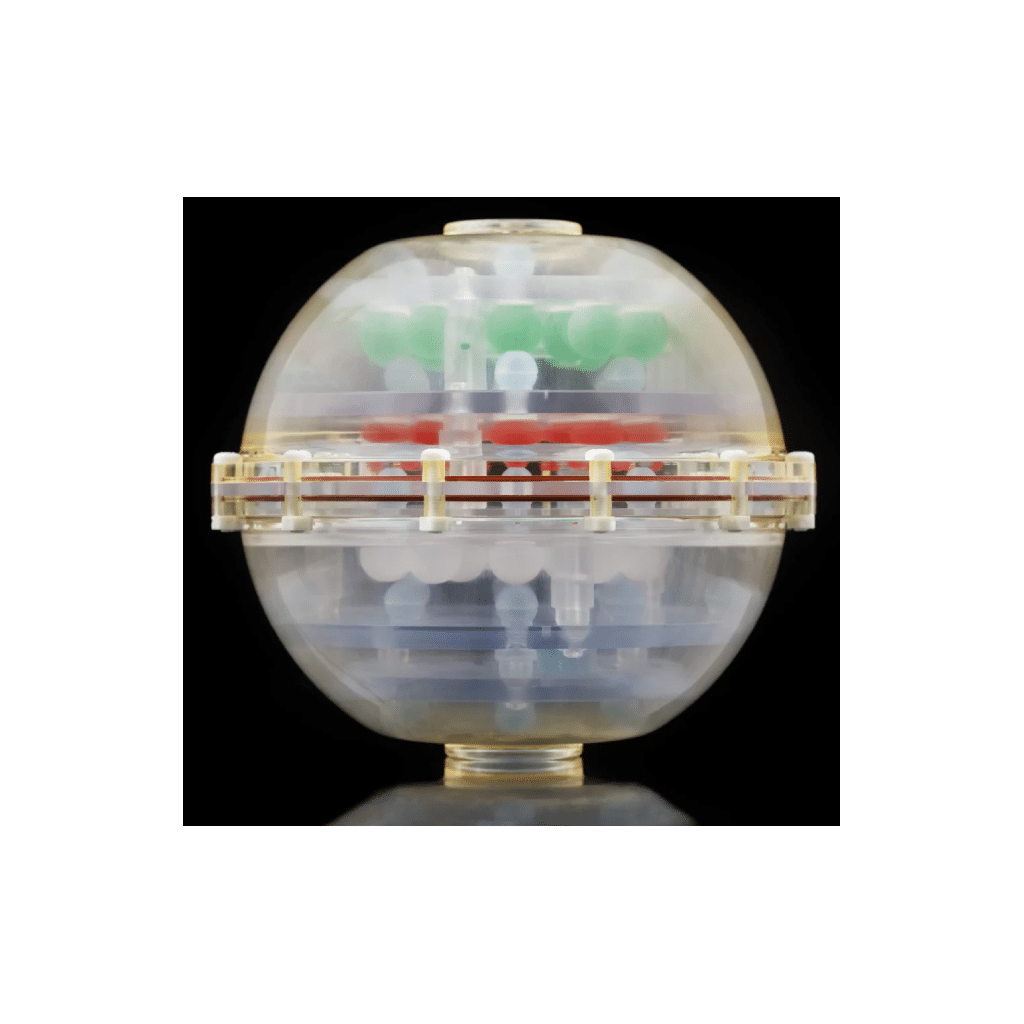
\includegraphics[width=0.75\linewidth]{imgs/mri_system_phantom/Premium-System-Phantom.png}
\caption{\textbf{The QalibreMD NIST/ISMRM System Standard Model 130 hardware
phantom.} The spherical water-filled housing (100 mm internal radius)
contains T1, T2, and PD contrast arrays, each consisting of 14
doped-solution spheres arranged in concentric rings at fixed axial
positions, plus a fiducial grid for registration. Its calibrated T1 (24
ms -- 1.9 s) and T2 (87 ms -- 2.8 s) ranges at 3 T span the full
physiological tissue window, making it the standard reference device for
quantitative MRI system validation. Image reproduced from
\href{https://qmri.com/product/premium-system-phantom/}{Caliber MRI}.}
\label{fig:premium-system-phantom}
\end{figure}

The relaxation values are field-strength-dependent, so separate
reference values are provided for 1.5 T and 3 T. The user manual also
distinguishes between legacy and modern serial-number classes; both sets
of reference values are included in the library.

\begin{center}\rule{0.5\linewidth}{0.5pt}\end{center}

\hypertarget{design-goals-and-architecture}{%
\section{Design goals and
architecture}\label{design-goals-and-architecture}}

A digital twin of this phantom is needed for two reasons. First, it
provides a ground-truth environment for RL training: the agent needs to
query a simulator that returns physically meaningful signals and can
report the true tissue parameters for reward computation. Second, it
must be \textbf{flexible}: the RL training loop needs to randomise pose,
inject noise, and jitter reference values across episodes without
modifying library code. Different experiments also require different
phantom sections or resolution.

The library is structured around a single contract: a
\texttt{PhantomConfig} struct that carries everything the builder needs,
passed to a single function \texttt{build\_phantom} that returns a
\texttt{KomaMRI.Phantom}. The phantom can then be fed directly to
\texttt{KomaMRI.simulate}. This design was chosen deliberately over a
mutable phantom object or a collection of keyword arguments as the
config is serialisable, diffable, and reproducible (the RNG seed is
embedded), and the builder has no hidden state. This is useful for
comparing different RL runs and also simplifies the Python-Julia
boundary used by the training code.

The pipeline from config to simulation is:

\begin{verbatim}
PhantomConfig
    |
    +-- sphere_descriptors(:T1, cfg)
    +-- sphere_descriptors(:T2, cfg)   one SphereDescriptor per contrast sphere
    +-- sphere_descriptors(:PD, cfg)   (geometry + material, no voxels yet)
    +-- sphere_descriptors(:fiducials)
    |
    +-- voxelise_sphere(d, delta_x)    -> KomaMRI.Phantom per sphere
    |
    +-- build_background_water(cfg)    -> KomaMRI.Phantom (water housing, sphere cutouts)
    |
    +-- apply_transform!(obj, rotation, translation)
    |
    +-- apply_per_spin_noise!(obj, augment, rng) -> KomaMRI.Phantom (ready for simulate())
\end{verbatim}

The two-stage design --- descriptors first, voxels second --- means all
geometry and material decisions happen before any memory is allocated
for spin arrays. Descriptors are also individually modifiable and
removable: you can simulate only a subset of the 14 spheres per plate,
with the water housing automatically filling the vacated volume. Because
each descriptor carries its physical centre coordinate,
\texttt{sphere\_descriptor\_pixels} can convert those centres directly
to pixel indices in the reconstructed image --- using the same
DC-at-centre convention as \texttt{kspace\_to\_image} --- simplifying
ROI extraction after reconstruction.

\begin{center}\rule{0.5\linewidth}{0.5pt}\end{center}

\hypertarget{geometry}{%
\section{Geometry}\label{geometry}}

The geometry implementation is judged by whether it preserves the
reconstructed sphere measurements, not by whether every background-water
spin is represented exactly.

\hypertarget{sphere-voxelisation}{%
\subsection{Sphere voxelisation}\label{sphere-voxelisation}}

Each sphere is voxelised on a cubic grid at spacing
\texttt{delta\_x\ =\ voxel\_size\_mm\ *\ 1e-3} metres. A spin is
included if its grid point falls within the sphere radius:

\[
(x_i - c_x)^2 + (y_i - c_y)^2 + (z_i - c_z)^2 \leq r^2
\]

The grid is constructed by iterating over the bounding box
\texttt{{[}c\ -\ r,\ c\ +\ r{]}} on each axis. For a typical 15 mm
radius sphere at 2 mm voxels this produces around 500 spins per sphere.
Across all three contrast plates (42 spheres), the combined spin count
at 2 mm voxels is \textasciitilde9,100, occupying \textasciitilde570 KB
(8 Float64 fields per spin:
\(x, y, z, \rho, T_1, T_2, T_2^*, \Delta\omega\)), small enough that the
full set fits comfortably in memory and the per-step simulate call is
fast.

\hypertarget{slicing}{%
\subsection{Slicing}\label{slicing}}

For 2D imaging experiments, only spins within a thin axial slab need to
be simulated, reducing the spin count, and therefore simulation time,
substantially. A \texttt{Slab} is defined by a centre point
\(\mathbf{c}\), a unit normal \(\hat{n}\), and a thickness \(t\). A spin
at position \(\mathbf{p}\) is included if its signed distance from the
midplane satisfies:

\[
|(\mathbf{p} - \mathbf{c}) \cdot \hat{n}| \leq t/2
\]

The normal defaults to \(\hat{z}\) but any orientation is supported. A
0.1 \(\mu\)m tolerance is applied at the boundary to avoid floating-point
rejections of on-edge voxels. At 1 mm voxels, a 5 mm axial slab centred
on the T1 plate retains \textasciitilde33,000 of the full phantom's
\textasciitilde4.2 million spins, a \textbf{\(128\times\) reduction}. This
matches the excited volume of a slice-selective RF pulse without needing
to encode one explicitly.

\hypertarget{pose-transforms}{%
\subsection{Pose transforms}\label{pose-transforms}}

\texttt{apply\_transform!} rotates and translates all spin positions by
the Euler XYZ rotation and translation specified in
\texttt{PhantomConfig.rotation} and \texttt{translation\_mm}. The
rotation matrix is built from three successive Rx, Ry, Rz
multiplications. The transform is applied after voxelisation and before
augmentation noise so that the sphere geometry is exact before any
stochastic perturbation. This was designed to make it easy to reset the
phantom and reduce overfitting.

\hypertarget{background-water}{%
\subsection{Background water}\label{background-water}}

The housing is voxelised as a 100 mm-radius sphere with
\texttt{water\_voxel\_size\_mm} spacing (defaulting to
\texttt{voxel\_size\_mm}), with all contrast and fiducial sphere volumes
cut out by the negated form of the squared-distance test used for
voxelisation. The water housing is by far the largest spin population,
yet it is not a quantity the phantom exists to measure, so it is the
natural place to trade fidelity for simulation speed. We do this by
increasing \texttt{water\_voxel\_size\_mm} to coarsen the grid, thus
reducing the spin count. We then reweight each spin's proton density by
\texttt{(water\_dx\ /\ sphere\_dx)³}. This conserves the total water
magnetisation, so the bulk water signal amplitude is correct regardless
of the coarsening factor.

This coarsening must also handle anisotropic resolution as slices are
typically thick (3--8 mm) relative to the in-plane resolution (1--2 mm).
So, when a slice is selected the housing is projected onto a grid of
stacked plane-sheets (\texttt{water\_throughplane\_voxel\_size\_mm}
apart). Again, these are re-weighted to conserve total magnetisation.

The figure below quantifies the fidelity--cost trade for an IR-SE-2D
acquisition.

\begin{figure}
\centering
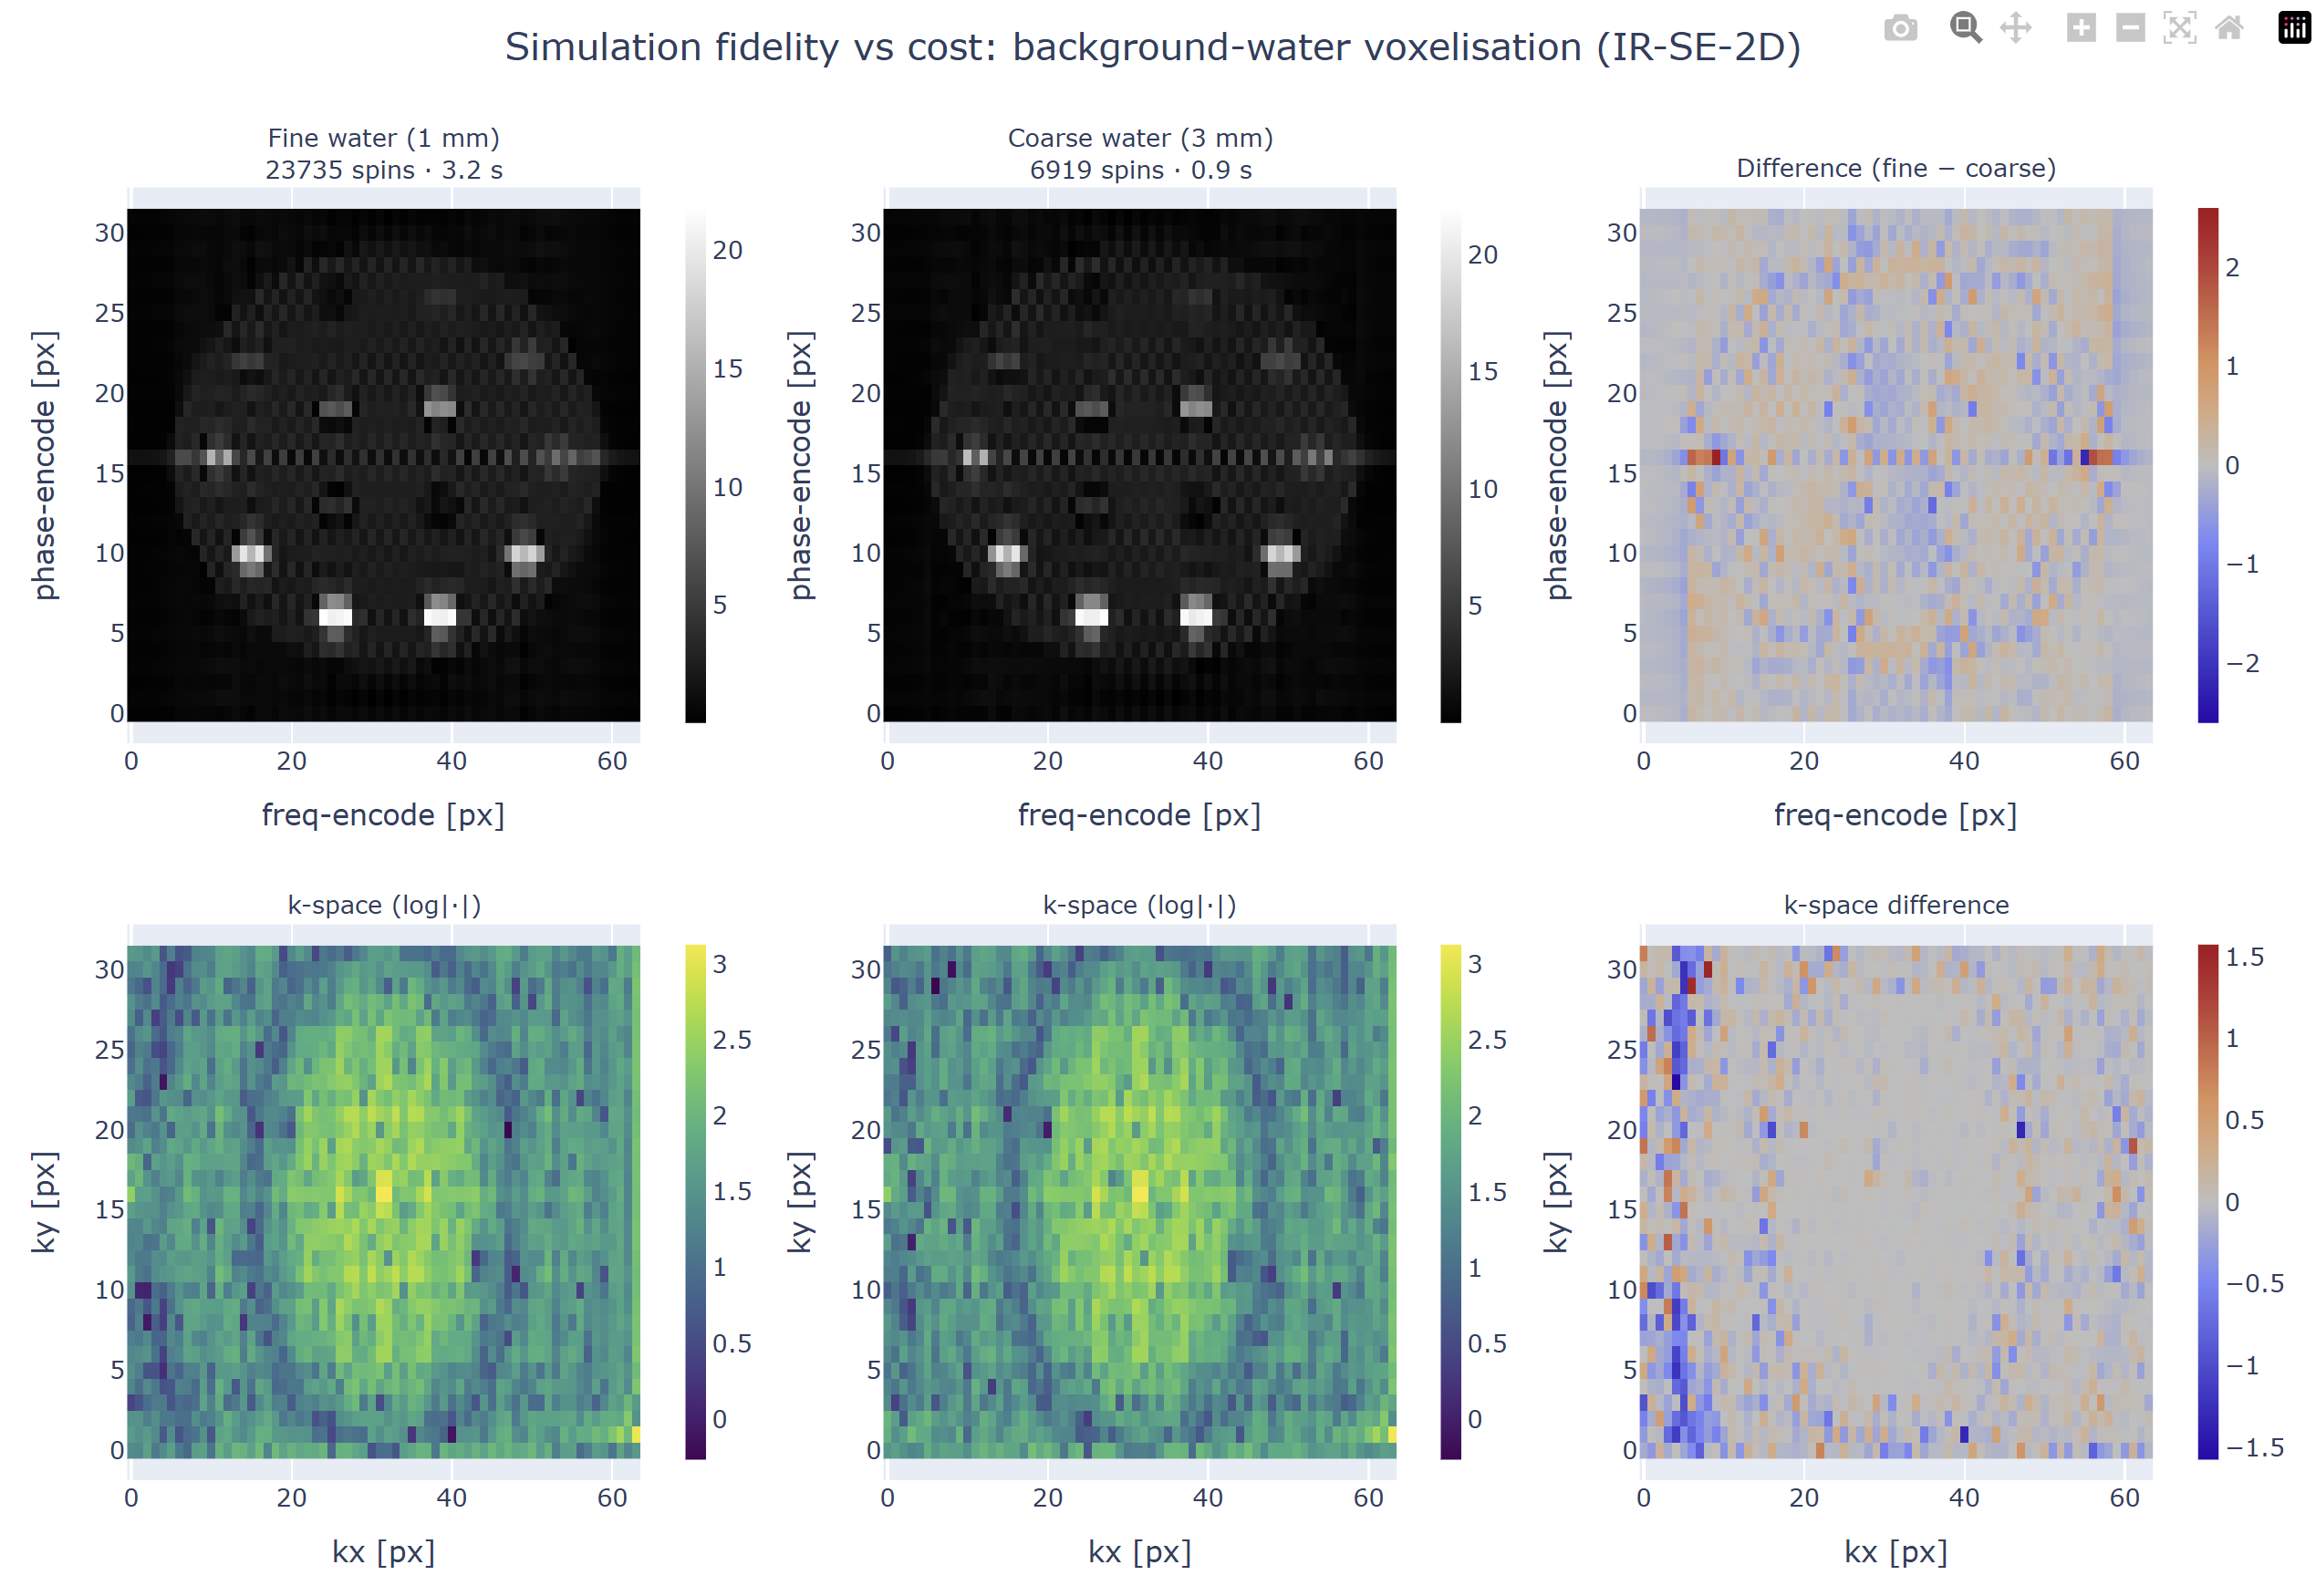
\includegraphics[width=\linewidth]{imgs/mri_system_phantom/water_voxel_fidelity.png}
\caption{\textbf{Fidelity--cost trade-off of background-water voxelisation.} The
same IR-SE-2D acquisition (TI/TE/TR = 400/80/1500 ms, \(32\times64\), FOV 0.2 m)
is simulated through two phantoms differing \emph{only} in
background-water discretisation. \textbf{Top row:} magnitude images;
\textbf{bottom row:} log-magnitude k-space; \textbf{right column:} fine
- coarse difference. The coarse 3 mm grid uses \textbf{6,919 vs 23,735
spins} (\(3.4\times\) fewer) and is \textbf{\textasciitilde\(3.4\times\) faster to
simulate} (\(0.9 \pm 0.1\) s vs \(3.2 \pm 0.6\) s, mean \(\pm\) std over 20 runs). The
total integrated signal (k-space DC) changes by only \textbf{0.35\%},
confirming the PD reweighting conserves the bulk water signal. The
visible residual is low-amplitude and concentrated at
high-spatial-frequencies. This figure and every number quoted in this
section are reproduced by running
\texttt{examples/compare\_water\_coarseness.jl}, which ships with the
library; the timings are wall-clock means over 20 repeats and will vary
with hardware.}
\label{fig:water-voxel-fidelity}
\end{figure}

Conserving the bulk water signal is necessary but not sufficient. The
k-space DC term changes by only 0.35\%, but the phantom is used to
measure the sphere signals. Using the
\texttt{sphere\_descriptor\_pixels} mapping from §1, the single
centre-pixel coarse-vs-fine NRMSE at the \(32\times64\) matrix is \textbf{3.7\%}.

The larger single-pixel error reflects where the coarse grid differs
from the fine one. Reweighting preserves the amount of water, but not
the exact water/sphere boundary: the 3 mm water grid stair-steps the
sphere cut-outs, changing high-spatial-frequency edge content while
leaving low-frequency k-space essentially unchanged. The boundary error
is on the scale of the reconstructed pixels here: for a 200 mm FOV and
\(32\times64\) matrix, the spacing is 6.25 mm in phase encode and 3.125 mm in
frequency encode. After band-limited reconstruction, this boundary
mismatch appears as a slightly different Gibbs-ringing pattern around
the spheres.

Most of this error is concentrated in the near-null spheres at this
inversion time, especially T1-spheres 13-14, whose signals move by about
9\%, while the bright spheres change by \(\leq 0.7\%\). This is expected because
the ringing leakage is approximately additive, set mostly by the
surrounding bright water.

If the sphere signal is measured as a small central ROI rather than a
single point sample, the error falls to \textbf{1.5\%} for a \(3\times3\) ROI.
This is the more relevant operational metric for an ROI-based phantom
readout; the single-pixel value remains useful as a worst-case
sensitivity measure because it exposes pixel-phase effects, Gibbs
oscillation, and sub-pixel centre rounding.

The same pattern strengthens at \(64\times64\): with unchanged spin counts and DC
term, the errors rise to \textbf{7.6\%} for a single centre pixel and
\textbf{2.3\%} for the \(3\times3\) ROI, consistent with a wider k-space window
admitting more of the edge mismatch.

Because the discrepancy is carried by truncation side-lobes, it can be
suppressed at reconstruction. The library provides a 2-D Hamming window
through \texttt{hamming\_window\_2d} and
\texttt{kspace\_to\_image(...;\ hamming=true)}. As derived in the
background chapter, this reduces the PSF side-lobes from -13 dB to -43
dB, at the cost of a wider main lobe.

\begin{figure}
\centering
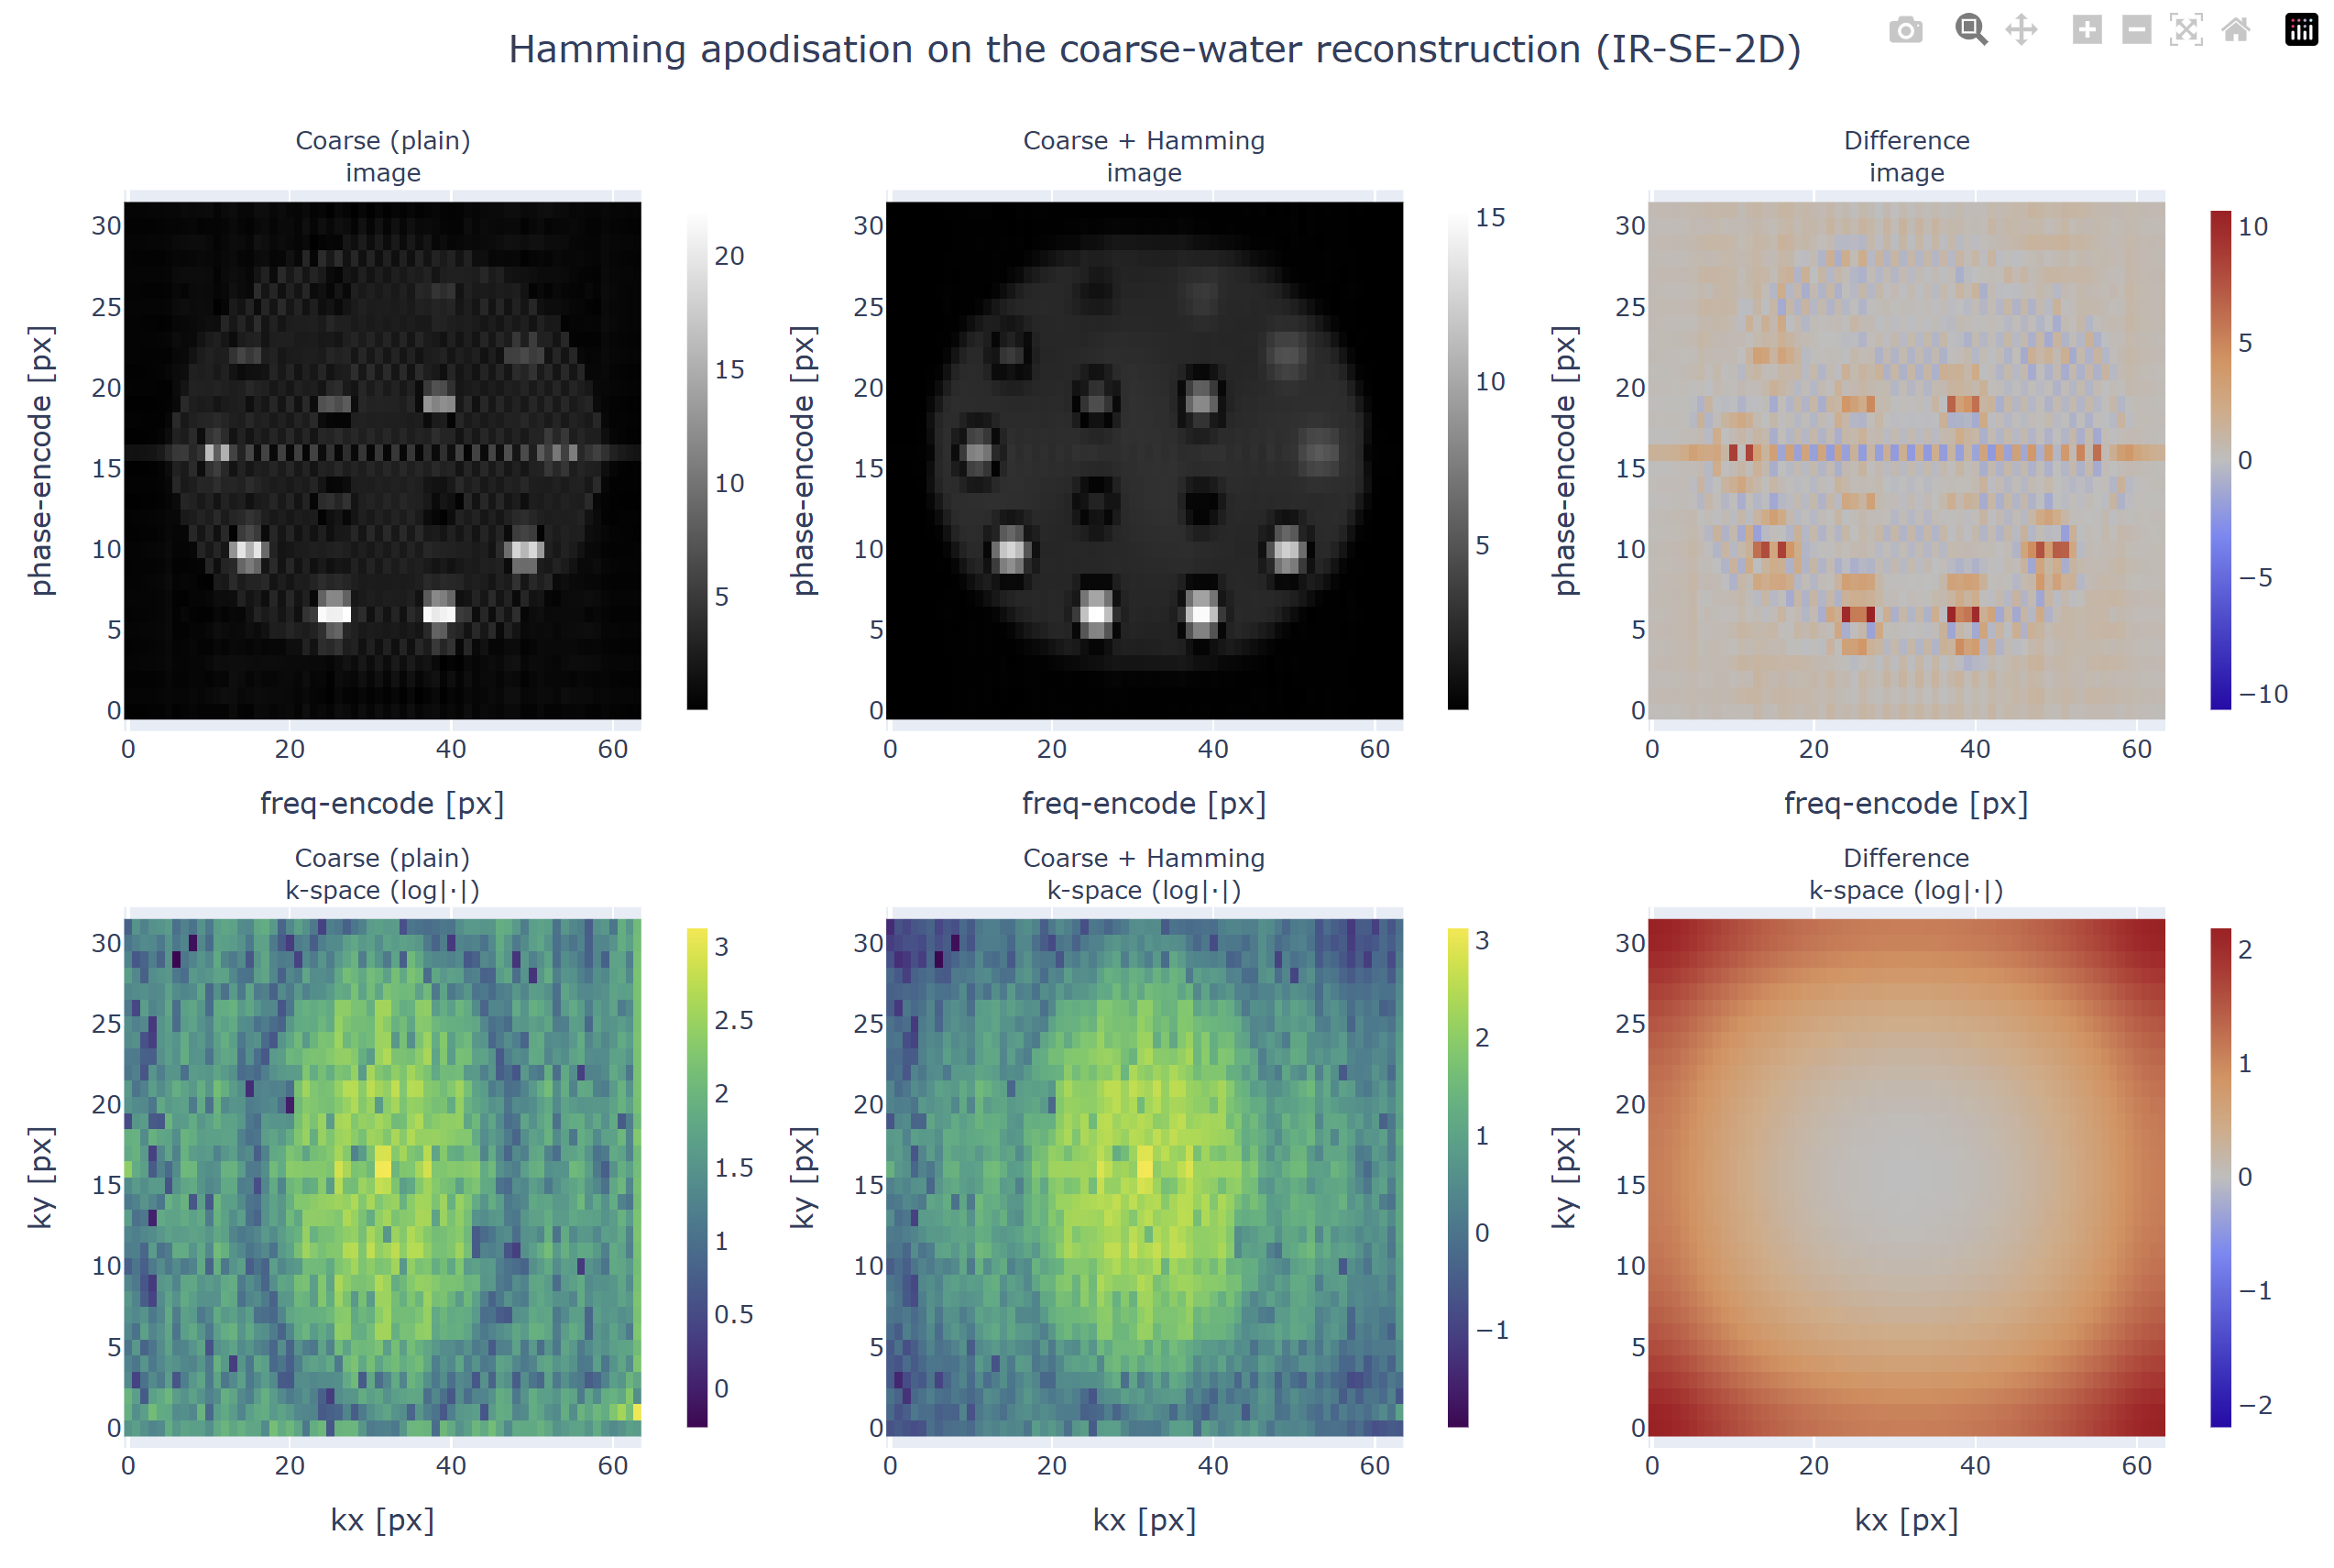
\includegraphics[width=\linewidth]{imgs/mri_system_phantom/hamming_phantom_diff.png}
\caption{\textbf{Effect of Hamming apodisation on one reconstruction.} A
coarse-water phantom reconstructed without a Hamming window (left), with
a 2-D Hamming window (centre), and their difference (right). The top row
shows magnitude images; the bottom row shows k-space after the
corresponding reconstruction weighting. The window down-weights outer
k-space, visible as the darkened periphery of the centre k-space panel.
This widens the PSF main lobe, slightly blurring the spheres, but
strongly suppresses ringing side-lobes. The difference is localised to
sphere edges and high-frequency k-space, consistent with suppression of
truncation ringing rather than a change in the smooth low-frequency
signal. Produced by \texttt{examples/hamming\_apodisation.jl}.}
\label{fig:hamming-phantom-diff}
\end{figure}

Reconstructing both grids with the Hamming window reduces the
single-pixel coarse-vs-fine NRMSE by four-fold, from \textbf{3.7\% to
0.9\%}. This confirms that the single-pixel discrepancy was dominated by
truncation ringing. The \(3\times3\)-ROI error improves more modestly, from
\textbf{1.5\% to 1.1\%}, because ROI averaging already cancels much of
the oscillatory side-lobe structure. Apodisation and spatial averaging
therefore suppress largely the same error component, rather than
providing independent gains. The remaining \(\approx 1.1\%\) is the residual
coarse-grid discrepancy under this ROI-based measurement protocol.

The Hamming window is a reconstruction-side element-wise multiplication
and costs only a fraction of a millisecond, so it does not affect the
roughly \(3\times\) simulation speed-up from the coarse grid. Its cost is
resolution, through the wider PSF main lobe.

A natural future improvement is a boundary-aware water grid: keep the
smooth water bulk coarse, but voxelise a thin shell around the housing
surface and sphere cut-outs at fine resolution so that coarsening no
longer changes the boundary geometry.

\begin{center}\rule{0.5\linewidth}{0.5pt}\end{center}

\hypertarget{material-tables}{%
\section{Material tables}\label{material-tables}}

The relaxation values are read from four module-level constants defined
from the phantom manual:

\begin{longtable}[]{@{}lll@{}}
\toprule
\begin{minipage}[b]{0.34\columnwidth}\raggedright
Constant\strut
\end{minipage} & \begin{minipage}[b]{0.30\columnwidth}\raggedright
Spheres\strut
\end{minipage} & \begin{minipage}[b]{0.27\columnwidth}\raggedright
Source\strut
\end{minipage}\tabularnewline
\midrule
\endhead
\begin{minipage}[t]{0.34\columnwidth}\raggedright
\texttt{T1\_ARRAY{[}:T3{]}} / \texttt{{[}:T15{]}}\strut
\end{minipage} & \begin{minipage}[t]{0.30\columnwidth}\raggedright
14 T1-plate spheres\strut
\end{minipage} & \begin{minipage}[t]{0.27\columnwidth}\raggedright
NiCl\(_2\) recipe, manual table, Serial Number \(\geq\) 0042\strut
\end{minipage}\tabularnewline
\begin{minipage}[t]{0.34\columnwidth}\raggedright
\texttt{T1\_ARRAY\_LEGACY{[}:T3{]}} / \texttt{{[}:T15{]}}\strut
\end{minipage} & \begin{minipage}[t]{0.30\columnwidth}\raggedright
same spheres\strut
\end{minipage} & \begin{minipage}[t]{0.27\columnwidth}\raggedright
manual table, SN pre-0042 (different values)\strut
\end{minipage}\tabularnewline
\begin{minipage}[t]{0.34\columnwidth}\raggedright
\texttt{T2\_OF\_T1\_ARRAY}\strut
\end{minipage} & \begin{minipage}[t]{0.30\columnwidth}\raggedright
T2 companions for T1 plate\strut
\end{minipage} & \begin{minipage}[t]{0.27\columnwidth}\raggedright
same manual table\strut
\end{minipage}\tabularnewline
\begin{minipage}[t]{0.34\columnwidth}\raggedright
\texttt{T2\_ARRAY{[}:T3{]}} / \texttt{{[}:T15{]}}\strut
\end{minipage} & \begin{minipage}[t]{0.30\columnwidth}\raggedright
14 T2-plate spheres\strut
\end{minipage} & \begin{minipage}[t]{0.27\columnwidth}\raggedright
MnCl\(_2\) recipe\strut
\end{minipage}\tabularnewline
\begin{minipage}[t]{0.34\columnwidth}\raggedright
\texttt{T1\_OF\_T2\_ARRAY}\strut
\end{minipage} & \begin{minipage}[t]{0.30\columnwidth}\raggedright
T1 companions for T2 plate\strut
\end{minipage} & \begin{minipage}[t]{0.27\columnwidth}\raggedright
same manual table\strut
\end{minipage}\tabularnewline
\begin{minipage}[t]{0.34\columnwidth}\raggedright
\texttt{PD\_FRACTIONS}\strut
\end{minipage} & \begin{minipage}[t]{0.30\columnwidth}\raggedright
14 PD-plate spheres\strut
\end{minipage} & \begin{minipage}[t]{0.27\columnwidth}\raggedright
proton density fractions\strut
\end{minipage}\tabularnewline
\begin{minipage}[t]{0.34\columnwidth}\raggedright
\texttt{BACKGROUND\_WATER}\strut
\end{minipage} & \begin{minipage}[t]{0.30\columnwidth}\raggedright
housing water\strut
\end{minipage} & \begin{minipage}[t]{0.27\columnwidth}\raggedright
distilled water at \(20^{\circ}\text{C}\)\strut
\end{minipage}\tabularnewline
\bottomrule
\end{longtable}

The T1 range at 3 T spans two decades: 23 ms to 1.84 s for the NiCl\(_2\)
plate, covering the full range of biological tissue T1 values from white
matter to cerebrospinal fluid. The T2 range spans \textasciitilde87 ms
to 2.76 s. These wide ranges are why the phantom is used for system
validation and make it useful for RL training: to ensure the learned
policies can produce reliable estimates across the full physiological
range.

The \texttt{serial\_number\_class} field switches the T1 table between
current and legacy recipes. All reference values are currently fixed at
\(20^{\circ}\text{C}\); the manual includes temperature-correction
graphs, but these are not yet implemented.

\textbf{Accuracy caveats.} Two entries are approximate: PD-plate T1/T2
values (\texttt{pd\_t1}, \texttt{pd\_t2}) use bulk water regardless of
proton-density fraction (the manual does not tabulate per-sphere
relaxation for the PD plate), and fiducial relaxation values
(\texttt{FIDUCIAL\_PROPS}) are generic CuSO\(_4\) placeholders not verified
against any calibration record. Neither affects the T1- or T2-plate
experiments, but both should be replaced before any simulation-to-real
comparison involving the PD plate or fiducial grid.

\begin{center}\rule{0.5\linewidth}{0.5pt}\end{center}

\hypertarget{augmentation}{%
\section{Augmentation}\label{augmentation}}

\texttt{AugmentConfig} enables domain randomisation for RL training. All
fields default to zero. When non-zero values are provided,
\texttt{apply\_per\_spin\_noise!} draws from the relevant distributions
using the config's \texttt{rng\_seed}:

\begin{longtable}[]{@{}ll@{}}
\toprule
\begin{minipage}[b]{0.44\columnwidth}\raggedright
Field\strut
\end{minipage} & \begin{minipage}[b]{0.50\columnwidth}\raggedright
Effect\strut
\end{minipage}\tabularnewline
\midrule
\endhead
\begin{minipage}[t]{0.44\columnwidth}\raggedright
\texttt{T1\_sigma\_rel}\strut
\end{minipage} & \begin{minipage}[t]{0.50\columnwidth}\raggedright
Multiplies each sphere's T1 by \texttt{exp(sigma*z)} where
\texttt{z\ \textasciitilde{}\ N(0,1)}, drawn once per sphere\strut
\end{minipage}\tabularnewline
\begin{minipage}[t]{0.44\columnwidth}\raggedright
\texttt{T2\_sigma\_rel}\strut
\end{minipage} & \begin{minipage}[t]{0.50\columnwidth}\raggedright
Same for T2\strut
\end{minipage}\tabularnewline
\begin{minipage}[t]{0.44\columnwidth}\raggedright
\texttt{PD\_sigma\_abs}\strut
\end{minipage} & \begin{minipage}[t]{0.50\columnwidth}\raggedright
Adds \texttt{N(0,\ sigma\^{}2)} to each spin's proton density\strut
\end{minipage}\tabularnewline
\begin{minipage}[t]{0.44\columnwidth}\raggedright
\texttt{position\_sigma\_mm}\strut
\end{minipage} & \begin{minipage}[t]{0.50\columnwidth}\raggedright
Adds \texttt{N(0,\ sigma\^{}2)} to each spin's (x, y, z) position
independently\strut
\end{minipage}\tabularnewline
\begin{minipage}[t]{0.44\columnwidth}\raggedright
\texttt{B0\_sigma\_Hz}\strut
\end{minipage} & \begin{minipage}[t]{0.50\columnwidth}\raggedright
Adds \texttt{N(0,\ sigma\^{}2)} per-spin off-resonance, stored in \(\Delta w\)
(rad/s after \(\times 2\pi\))\strut
\end{minipage}\tabularnewline
\begin{minipage}[t]{0.44\columnwidth}\raggedright
\texttt{drop\_sphere\_p}\strut
\end{minipage} & \begin{minipage}[t]{0.50\columnwidth}\raggedright
Drops each sphere independently with Bernoulli probability p before
voxelisation\strut
\end{minipage}\tabularnewline
\bottomrule
\end{longtable}

The T1/T2 jitter is applied at the sphere level (one draw per sphere,
not per spin) to simulate manufacturing variability in the doping
concentration. Of the fields above, only \texttt{T1\_sigma\_rel} and
\texttt{T2\_sigma\_rel} were used in the experiments of this work; the
remaining fields are implemented for completeness but were not
exercised.

The \texttt{rng\_seed} is the only source of stochasticity: fixing it
makes \texttt{build\_phantom} deterministic, so the same configuration
always produces the same phantom. Fixing the seed reproduces the exact
same phantom, making evaluation runs reproducible. Incrementing it each
training episode draws a statistically independent phantom, preventing
the agent from memorising a fixed configuration.

\begin{center}\rule{0.5\linewidth}{0.5pt}\end{center}

\hypertarget{komamri-integration}{%
\section{KomaMRI integration}\label{komamri-integration}}

\texttt{MRISystemPhantom.jl} is built entirely on top of
\texttt{KomaMRI.jl} and returns standard \texttt{KomaMRI.Phantom}
objects. The whole phantom is assembled using a single operation: the
concatenation operator \texttt{+} on \texttt{Phantom}. Each voxelised
sphere becomes a small \texttt{Phantom}, the spheres of each T1, T2 and
PD plate are concatenated into that plate, the three plates are
concatenated into a sphere stack, and finally the water background is
concatenated on top. The result is a single array of spins with
heterogeneous relaxation values, which is exactly what
\texttt{KomaMRI.simulate} expects.

Because the output is an ordinary \texttt{KomaMRI.Phantom}, existing
KomaMRI features work out of the box, such as the interactive plotting
tools which are used extensively in the example scripts.

The matching scanner is obtained from \texttt{scanner\_for\_field(cfg)},
which returns a \texttt{Scanner} with B0 set to 3.0 T for \texttt{:T3}
or 1.5 T for \texttt{:T15}. Pairing a phantom with a \texttt{Scanner} of
a different B0 silently produces the wrong relaxation values - a mistake
the author made in practice - so this helper exists to make the coupling
explicit.

\begin{center}\rule{0.5\linewidth}{0.5pt}\end{center}

\hypertarget{library-availability}{%
\section{Library availability}\label{library-availability}}

\texttt{MRISystemPhantom.jl} is developed as a standalone open-source
Julia package at \texttt{github.com/ArthurAllilaire/MRISystemPhantom.jl}
with API documentation hosted at
\texttt{arthurallilaire.github.io/MRISystemPhantom.jl}. The package
includes a complete test suite (\textasciitilde373 tests) and
documentation pages covering phantom construction, sequence design,
parameter fitting, and SNR diagnostics.

An independent, public library has several benefits: 1. It provides a
complete, tested forward pipeline --- phantom construction, sequence
generation, simulation, reconstruction, ROI extraction, and parameter
fitting --- rather than a set of experiment-specific scripts. 2. It
makes the methodology reproducible and extensible for other groups
working on quantitative MRI system validation or simulation-based
sequence optimisation. 3. It provides a reusable digital twin of a
widely deployed calibration device, so simulated methods can be checked
against known T1/T2 reference values before scanner deployment. 4. It
integrates directly with the Julia/KomaMRI ecosystem by returning
standard \texttt{KomaMRI.Phantom} and \texttt{Sequence} objects. 5. Its
example scripts provide runnable, educational references for phantom
construction, sequence design, parameter fitting, SNR calibration, and
the fidelity checks reported here.

\hypertarget{example-scripts}{%
\subsection{Example scripts}\label{example-scripts}}

The package ships a set of runnable, self-contained demonstration
scripts in \texttt{examples/}. Each exercises one slice of the public
API and writes interactive Plotly HTML into \texttt{src/assets/}.

\begin{itemize}
\tightlist
\item
  \texttt{plot\_phantom.jl}: renders the T1/T2/PD maps and slice cuts of
  the built phantom.
\item
  \texttt{plot\_fidelity\_phantoms.jl}: visualises the water-coarsening
  fidelity levels.
\item
  \texttt{t1\_mapping.jl}: runs a full IR-SE acquisition, reconstructs
  the image, extracts per-sphere ROIs and fits T1.
\item
  \texttt{conventional\_baseline.jl}: runs the conventional
  fixed-sequence baseline (IR/SE sweep plus fit for all 28 T1 \& T2
  contrast spheres).
\item
  \texttt{snr\_calibration.jl}: performs the NEMA MS-1 dual-acquisition
  SNR measurement.
\item
  \texttt{compare\_water\_coarseness.jl} and
  \texttt{hamming\_apodisation.jl}: produce the fidelity-vs-cost and
  apodisation figures (§2.3) along with the numbers quoted there.
\item
  \texttt{plot\_seqs.jl}: writes one interactive RF/gradient/ADC
  waveform plot per sequence into \texttt{src/assets/sequences/}.
  Sequences included: IR-SE (with and without crusher \& TR-spoiler
  variant), SE for T2 mapping, IR-TSE echo-train, and spoiled GRE.
\end{itemize}

Because the output is a standard
\texttt{KomaMRI.Phantom}/\texttt{Sequence}, these scripts rely only on
KomaMRI's own interactive plotting, with no bespoke visualisation code
in the library.

\begin{center}\rule{0.5\linewidth}{0.5pt}\end{center}
